%------------------------------------------------
\begin{frame}
\Huge{\centerline{Execution of Multi-Agent Systems}}
\end{frame}

%------------------------------------------------

\begin{frame}
\frametitle{Semantics of Computational Run }
\begin{block}{Definition}
	The execution of a 2APL multi-agent system with initial configuration $A_1,...,A_n, χ$ is the set of computation runs $CR(A_1,...,A_n, χ)$ of the 2APL transition system.
\end{block}


\begin{block}{Definition}
	A computation run $CR(s0)$ is a sequence $s_0,...$ where $s_i$ is a
configuration, and $∀i>0 : s_i−1 → s_i$ is a transition in the transition system.
\end{block}

\end{frame}


%------------------------------------------------

\begin{frame}
	\frametitle{Single-Agent Deliberation Cycle}
    \begin{figure}
      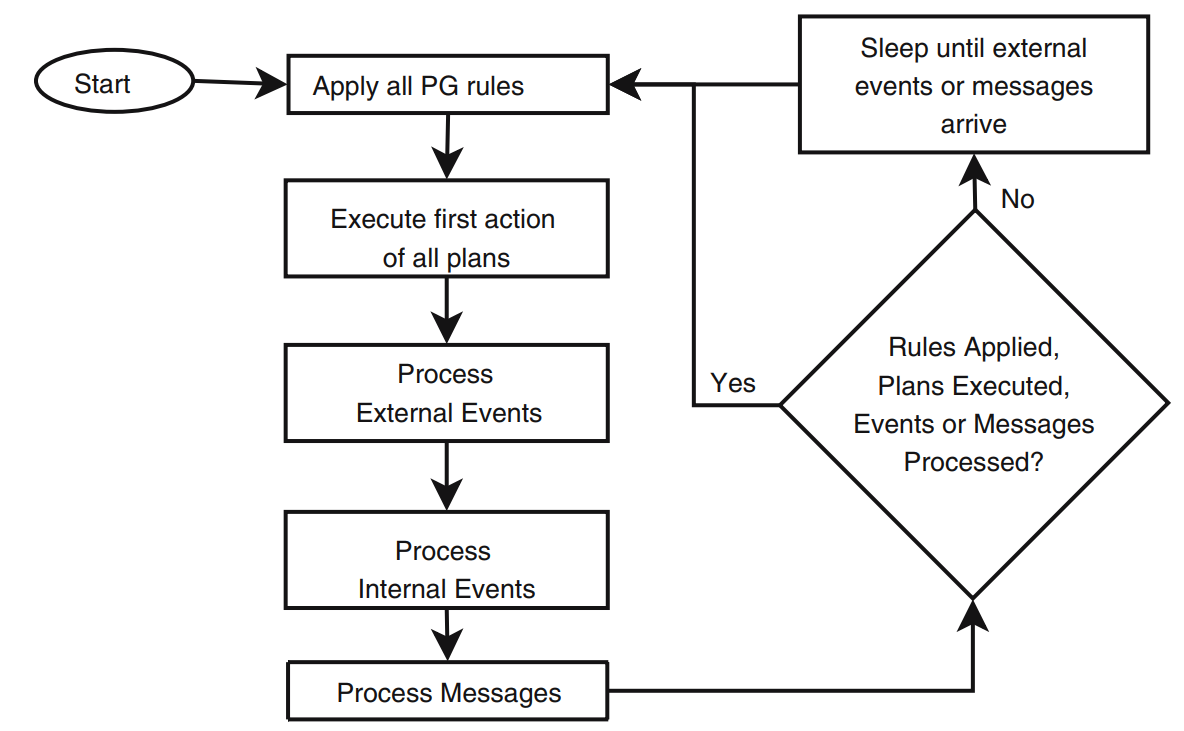
\includegraphics[width=1\textwidth]{deliberation-cycle-individual-2apl}}
    \end{figure}
\end{frame}